\section{Results}
We here show the results of a cortical layering on simulated data, human ex vivo data, and human in vivo data. We compare the extracted laminar signals for three different methods, the GLM, interpolation, and classification approach.

\subsection{Model Cortex}
The three different layer extraction methods were first applied to the modelled cortex, in order to estimate a point spread function of the method in ideal circumstances. The layer profiles of all layers were aligned and averaged \remove{(\texttt{nanmean})} and are shown in Figure~\ref{fig:pointspread} for both resolutions ($[0.5 $ mm$]^3$ and ($[1.0 $ mm$]^3$). The full unaveraged point spread functions are also shown in Supplementary Figure~\ref{fig:pointspreadall} in matrix form. The ideal PSF is a single peak of height one at the origin with no leakage to neighbouring layers.
\begin{figure}[ht]
	\centering
	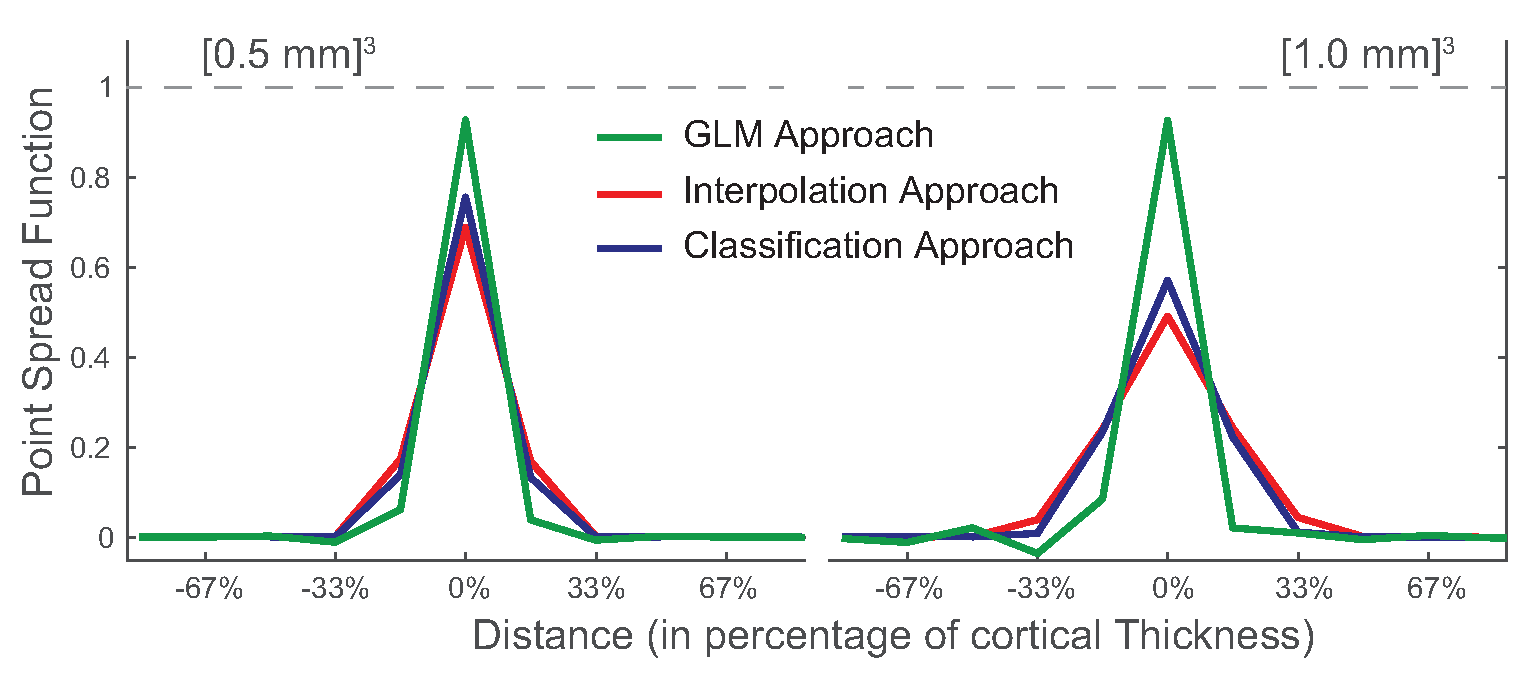
\includegraphics[width=1.\textwidth, clip=true]{./Chapters/03_GLM/./Images/PointSpread}
	\caption{The performance of the three different approaches of obtaining layer signal, represented as a point spread function (PSF) obtained on simulated data. An ideal PSF would be an unit peak at the origin. The results are shown for approximate resolutions of 0.5 mm and 1.0 mm, on the left and right respectively. The GLM approach has a sharper PSF and is able to retrieve more signal, but potentially at the cost of a small undershoot in neighbouring layers.}
	\label{fig:pointspread}
\end{figure}

For the 0.5 mm resolution volume \add{(i.e. one layer per voxel)}, the peak of the distribution for the GLM reaches 92,5\%, which is considerably higher than the 75.4\% for the classification approach and 68,7\% for the interpolation approach. This means that the latter two approaches respectively lose approximately a quarter and a third of the signal to neighbouring layers, as opposed to a only 7.5\% in the GLM approach. For all methods, the leakage is close to symmetrical. The small remaining asymmetries are likely to be related to a small imbalance in proportion of voxels with a positive and negative curvature.

Also for the 1.0 mm scenario, the PSF for the GLM approach is considerably sharper. The GLM approach peaks with 92.4\%, the classification approach with 56.9\%, and the interpolation approach with 49.0\%. As expected, the PSFs for the interpolation and classification approach are less sharp for coarser resolutions. Surprisingly, the GLM approach peaks higher, but this comes at a cost: several undershoots are visible in a sinc-like oscillating pattern. Effectively, this artificially boosts the peak signal by `stealing' it from other layers. \add{The spatial design matrix is more ill-conditioned as the number of layers is double the number of voxels over the thickness of the cortex.}

The same analysis was repeated without including the gradient estimate in the layering, and instead using a cubic polynomial approximation for the partial volume kernel \cite{Koopmans2011}. The resulting PSFs were identical up to 2\% margin, showing that incorporating this extra type of prior knowledge has merely marginal effects on the outcome.

\subsection{High resolution data}
The extracted profile of the high resolution data is shown in Figure~\ref{fig:exvivovolume}, together with an image of the data in which the region of interest is delineated. The structure of the cortex is clearly visible in the extracted profiles. It shows the intensity difference around the stria of Gennari. Additionally, towards the pial surface there is a drop in intensity of which the anatomical origin is unknown. Also note the sharp transition at the pial boundary, quickly dropping to almost zero. The average profiles look like accurate reflections of the ROI, but all methods performs roughly the same. It should be noted, however, that in all regions the GLM shows some oscillating behaviour which is likely to be artifactual to the method. This can easily be related to the sinc-like point spread function that was computed in the simulation. This effectively represents a kernel that is convolved with the true profile and thus shows the same oscillatory behaviour, much related to Gibbs ringing \cite{Gibbs1898}. In particular, the artifacts proliferate at the edges of the cortex, as they scale as a function of the differences between neighbouring layers.
\begin{figure}[ht]
\centering
\includegraphics[width=1.\textwidth, clip=true]{./Chapters/03_GLM/./Images/MichielData}
\caption{The layering, the regions of interest, and the extracted cortical profiles for three regions. While all three methods perform almost identically, there are small oscillations present in the profiles as produced by the GLM. Especially in the top layer, the peak is potentially mistakenly higher than both other methods suggest.}
\label{fig:exvivovolume}
\end{figure}

\subsection{MP2RAGE data}
The cortical profiles of the primary visual cortex for 11 subjects is shown for a variety of methods in Figure~\ref{fig:profileaverage}. First, the three main methods were compared based on the average over subjects. The error bars represent the standard error of the mean. The classification and interpolation approach both show smooth monotonically decreasing profiles for any number of layers. In all case, the GLM method estimates the WM signal to be higher and the CSF signal to be lower than both other methods. This could reflect a lower partial volume leakage to neighbouring layers, but may be indistinguishable from an edge enhancing artifact similar to the ones visible in the previous results. Without a gold standard, this cannot be assessed. In contrast to the two other methods, the GLM starts showing oscillating behaviour when the cortex is divided into more layers. \add{In particular, when the artifacts seem to increase dramatically when the number of layers is higher than the number of voxels.} While the average over subjects is still relatively smooth, the increasing standard errors already suggests higher subject specific differences. This is especially visible in the subject specific profiles (second row of Figure~\ref{fig:profileaverage}). The highly fluctuating individual profiles for 8 cortical layers is unlikely to reflect any true underlying anatomical variation. In general, no method seems to be able to extract anatomical details, such as the stripe of Gennari. Anecdotally, the stripe is visible in some subjects, but it does not survive the anatomical variation in combination with the sensitivity limitations of the layer extraction pipeline.

Lastly, we investigated the assumption of correlated noise in the volume. We varied the \change{FWHM}{correlation length} of an assumed Gaussian noise correlation, performed a generalised least squares regression, and investigated the average profiles. For $L_c= 0$ mm, the solution reduces to an ordinary least squares problem. It can be observed that for a small \change{FWHM}{correlation length} (1 mm), there is only a marginal difference with no correlated noise at all. With a larger \change{FWHM}{correlation length} (2 mm), all profiles become somewhat smoother, but for larger values (3 mm) results start to wildly fluctuate to the extent that they are uninterpretable. It can therefore be concluded that GLS should only be used with extreme care, and that the results with the tested covariance matrices show marginal improvements at best over OLS.
\begin{figure}[ht]
	\centering
	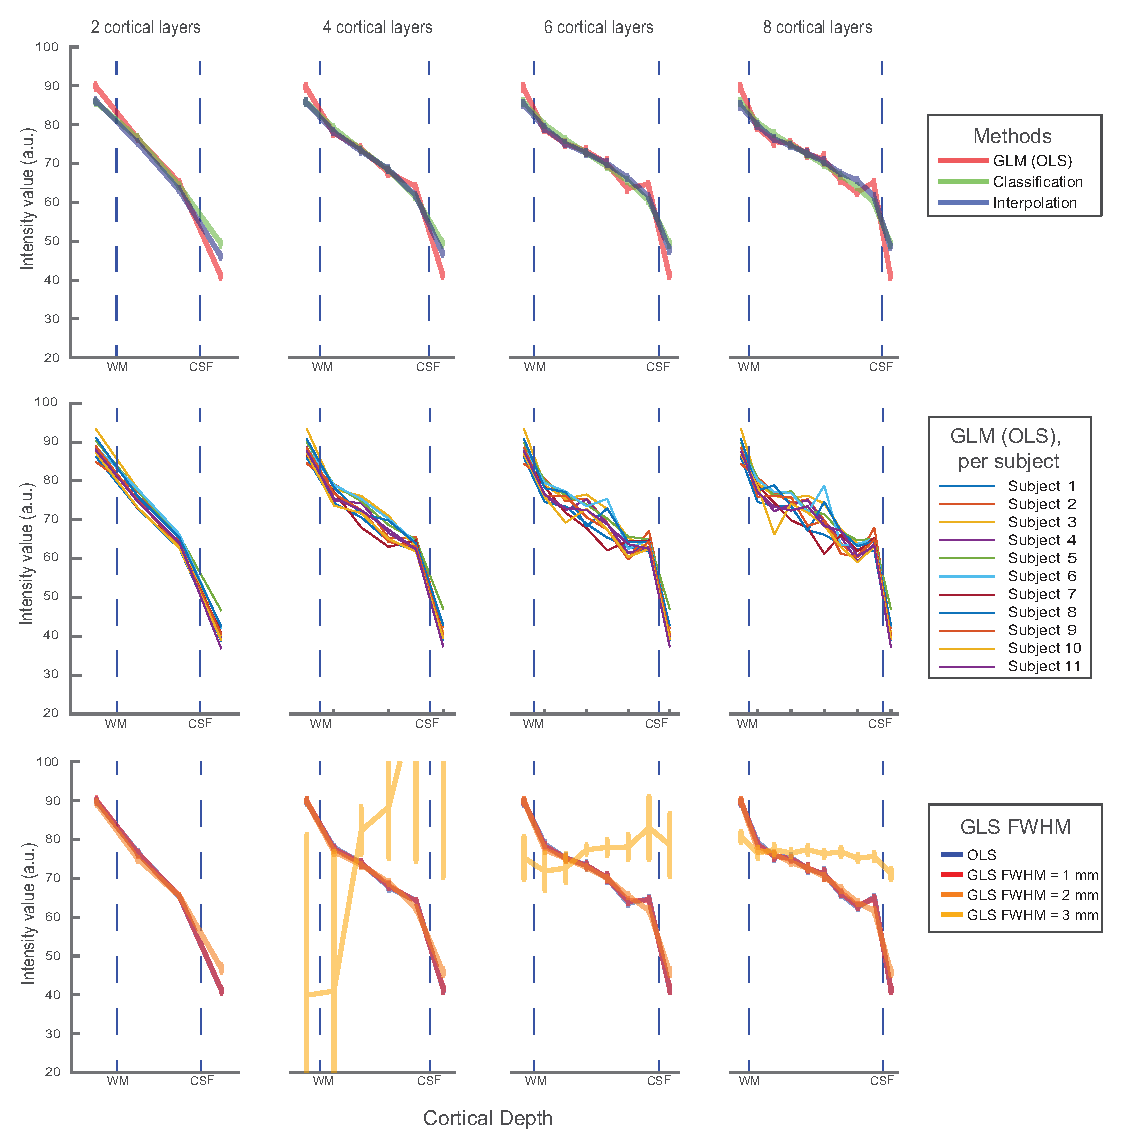
\includegraphics[width=0.9\textwidth, clip=true]{./Chapters/03_GLM/./Images/ProfileComparisons}
	\caption{The obtained profiles for a small piece of the primary visual cortex, based on 11 subjects, for a varying number of layers (columns). In the first row, the three different methods are compared. The second row shows the individual profiles for the GLM method, showing that the solution becomes unstable when higher numbers of layers are used. In the bottom row, different FWHMs are tested in a generalised least squares solution.}
	\label{fig:profileaverage}
\end{figure}
